\section{Model Representations}
\label{sec:representations}

The design of the \Treebeard{} compiler allows the implementation of different strategies for 
the in-memory representation of the model. The compiler currently has implementations for 
the three representations shown in Figure \ref{Fig:Representations}. The array and sparse 
representations are as proposed in \TreebeardOLD{}~\cite{Treebeard}. The reorg 
representation is the representation used by the RAPIDs library\cite{FIL}. 
The \textbf{array representation} is the simplest representation where the trees are stored in an array
in level order. The \textbf{sparse representation} stores the trees in a sparse format where 
memory is allocated only for nodes present in the tree and nodes contain pointers to their children. The \textbf{reorg representation}
interleaves the array representation of each tree in the model: all root nodes are stored first, then 
the left children of all the roots and so on. This representation was 
designed to improve memory coalescing when tree nodes are being loaded. 
\begin{figure}[htb]
  \centering
  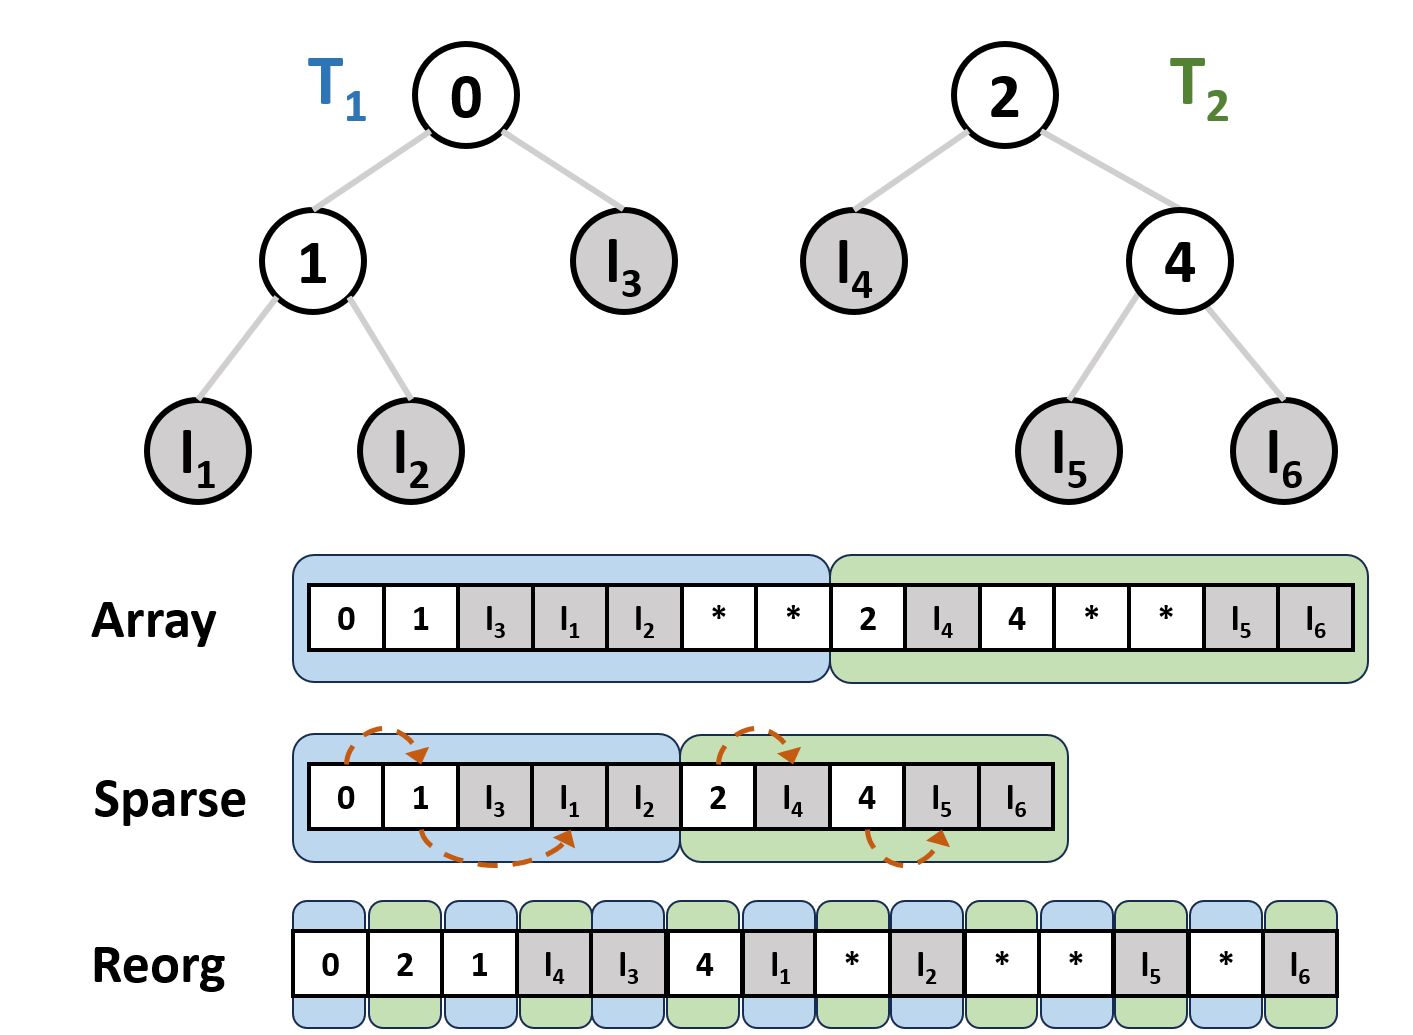
\includegraphics[width=0.7\linewidth]{figures/representations.png}
  \caption{The three representations supported by \Treebeard{}.}
  \label{Fig:Representations}
\end{figure}

We change the design of \TreebeardOLD{}~\cite{Treebeard} to
separate the implementation of representations from the rest of the compiler. This allows
us to implement representations as plugins to the compiler. We define an interface 
that representations implement. The code generator is implemented using
this interface thus hiding details of the actual representation from the core 
compiler. Crucially, the interface abstracts how and what buffers 
are allocated, how to move from a node to its child, how trees 
are cached, reading the value of leaves and how threshold and 
feature indices are read from the allocated buffers.
% The interface abstracts the following details. 
% \begin{itemize}
%   \item \textbf{Buffer allocation:} The representation object exposes methods that generate 
%   buffer allocations in the IR. 
%   \item \textbf{Moving to child nodes:} Given the value of the predicate at a node (or tile),
%   generate code to move to the appropriate child node of the current node.
%   \item \textbf{Leaf representation:} The interface abstracts determining whether the current
%   node is a leaf (which is needed to terminate walks) and how to get the value of the leaf
%   (which is needed to get a tree's prediction).
%   \item \textbf{Caching trees:} Since reading the trees into shared memory on GPU (or prefetching)
%   them on CPU require knowledge of the buffer layout, the task of generating caching code for trees
%   is delegated to the representation object. 
%   \item \textbf{Loading thresholds and feature indices:} The representation object provides MLIR 
%   rewrite patterns to lower operations that load thresholds and feature indices to LLVM IR. This
%   is necessary because the details of how to load the thresholds and feature indices from the model 
%   buffers is representation-specific.
% \end{itemize}

In summary, the representation interface abstracts the details of how the model is stored in memory
and allows the compiler to generate code without having to explicitly know the details of the
representation. This design allows us to implement new representations without changing the core
compiler infrastructure. Implementing the representations as plugins also allows us to reuse
the implementations across different lowering pipelines. 

% For example, the code for the array 
% and sparse representations is almost fully shared between the CPU and GPU lowering pipelines.   

\section{Caching}
\label{sec:caching}

% \begin{itemize}
%   \item The compiler exposes caching of both trees and input rows in a unified manner.
%   \item This is independent of the final target on which the inference is to be run.
%   \item The caching is done at the granularity of a tree or a row.
%   \item Caching is encoded in the mid-level IR using the \op{cacheTrees} and \op{cacheRows} operations. 
%   These operations are generated when the HIR lowered to MIR and \op{Cache()} is specified on an 
%   index variable in the schedule. While the HIR is being lowered and a cached index variable is 
%   encountered, the compiler generates a \op{cacheTrees} or \op{cacheRows} operation depending on 
%   whether the index variable is a tree or a batch index variable.
%   \TODO{Should we talk about how the lowering from HIR to MIR is actually implemented as a tree walk?}
%   \item The lowering of these ops is done by the target-specific code generator.
%   \item For the \op{cacheRows} operation, \Treebeard{} uses pre-implemented lowerings for both
%   CPU and GPU. This is possible because the input is currently assumed to be a dense 
%   array format. 
%   \item For the \op{cacheTrees} operation, the lowering is representation-specific.
%   Each representation provides a lowering to the target-specific code generator
%   to lower the \op{cacheTrees} op when that representation is used.
%   \item The cache operations are lowered to reads into shared memory while compiling to GPU 
%   and to prefetches while compiling to CPU.
% \end{itemize}

\Treebeard{} provides mechanisms to cache both trees and input rows 
on both the CPU and GPU. As described in Section \ref{sec:schedule}, 
the user can specify that the working set of an iteration of a loop
needs to be cached using the \op{cache} directive. 
% This provides a unified way to specify caching of both trees and input rows.
\Treebeard{} implements caching at the granularity of a tree or a row.

% \subsection{IR Representation of Caching}
Caching is encoded in the mid-level IR using the \op{cacheTrees} and \op{cacheRows} operations (Table \ref{Tab:IRSpecification}). 
% These operations are generated when the HIR lowered to MIR and \op{cache} is specified on an 
% index variable in the schedule. 
When the HIR is being lowered and a cached index variable is 
encountered, the compiler generates a \op{cacheTrees} or \op{cacheRows} operation depending on 
whether the index variable is a tree or a batch index variable.
\Treebeard{} also determines the working set of one iteration of the loop  
and generates a caching operation with the appropriate limits.

% Each of the caching operations take parameters that specify the set of trees or rows that need 
% to be cached. The caching operations are defined as follows. 
% \begin{itemize}
%   \item \textbf{\op{cacheTrees(forest, start, end)}:} This operation caches the trees in ensemble
%   \op{forest} from \op{start} to \op{end}. The trees are cached in the order in which they are
%   specified in the ensemble. 
%   \item \textbf{\op{cacheRows(data, start, end)}:} This operation caches the rows in the input 
%   array \op{data} from \op{start} to \op{end}. The rows are cached in the same order as in the
%   input array.
% \end{itemize} 

%\subsection{Lowering of Caching Operations}
When the MIR is lowered to LIR, the cache ops are lowered to target-specific code. Each of 
the two caching operations is lowered differently for the CPU and the GPU. On CPU, the cache operations are lowered to prefetches while
on the GPU they are lowered to reads into shared memory.

Lowering the \op{cacheRows} operation is straightforward
% \Treebeard{} uses pre-implemented lowerings for both
% CPU and GPU. This is possible 
because the input is currently assumed to be a dense
array format. The lowering for the \op{cacheRows} operation is 
implemented directly in the \Treebeard{} compiler as a series of 
coalesced loads into shared memory.

For the \op{cacheTrees} operation, the lowering is representation-specific. Each representation
provides a lowering to the target-specific code 
generator to lower the \op{cacheTrees} op.
%  However, the \Treebeard{} infrastructure does provide helpers 
% to generate caching code to cache contiguous regions of memory. These helpers are reused 
% as required across different representations. 
